\documentclass[11pt,a4paper]{article}
%DIF LATEXDIFF DIFFERENCE FILE
%DIF DEL sc_documentation_1-00.tex   Tue Feb 13 13:12:42 2018
%DIF ADD sc_documentation_1-10.tex   Tue Feb 13 13:59:59 2018

% font
\renewcommand{\familydefault}{\sfdefault}

%DIF 6d6
%DIF < 
%DIF -------
\usepackage[margin=0.8in]{geometry}
\usepackage[utf8]{inputenc}
\usepackage{amsmath}
\usepackage{amsfonts}
\usepackage{amssymb}
\usepackage[hidelinks]{hyperref}
\usepackage{float}

\usepackage{lipsum}% http://ctan.org/pkg/lipsum

%% Bibliography/references packages
\usepackage[comma]{natbib}
%%\bibliographystyle{agsm}
\bibliographystyle{dcu}

%% https://en.wikibooks.org/wiki/LaTeX/List_Structures
\usepackage{scrextend}

% tables, row colour
\usepackage{tabularx,colortbl}

% https://tex.stackexchange.com/questions/22751/how-to-force-table-caption-on-top
%\usepackage[tableposition=top]{caption}
\usepackage{float}
\floatstyle{plaintop}
\restylefloat{table}

% https://en.wikibooks.org/wiki/LaTeX/List_Structures
\usepackage{enumitem}


%% Report variables
\newcommand{\scname}{PRCO}
\newcommand{\dlatestv}{1.00}

%DIF 42a41-43
\definecolor{babyblueeyes}{rgb}{0.63, 0.79, 0.95} %DIF > 
\definecolor{ballblue}{rgb}{0.13, 0.67, 0.8} %DIF > 
 %DIF > 
%DIF -------
\usepackage{array,booktabs,arydshln,xcolor}
\usepackage{xcolor}% http://ctan.org/pkg/xcolor
\usepackage{fancyhdr}% http://ctan.org/pkg/fancyhdr
\fancypagestyle{main}{%
	\renewcommand{\headrulewidth}{2pt}
	\renewcommand{\headrule}{\hbox to\headwidth{%
%DIF 48c50
%DIF < 		\color{red}\leaders\hrule height \headrulewidth\hfill}}
%DIF -------
		\color{ballblue}\leaders\hrule height \headrulewidth\hfill}} %DIF > 
%DIF -------
	\renewcommand{\footrulewidth}{2pt}
	\renewcommand{\footrule}{\hbox to\headwidth{%
%DIF 51c53
%DIF < 		\color{red}\leaders\hrule height \headrulewidth\hfill}}
%DIF -------
		\color{ballblue}\leaders\hrule height \headrulewidth\hfill}} %DIF > 
%DIF -------
	
	%\fancyhf{}
	%\fancyhead[LE]{\textbf{\leftmark}}
	%\fancyhead[RE]{\textbf{\scname{}}}
	%\fancyhead[LO]{\textbf{\scname{}}}
	%\fancyhead[RO]{\textbf{\rightmark}}

	%\fancyfoot[LE]{\textbf{\thepage}}
	%\fancyfoot[RE]{\textbf{\scname{} Configuration Guide}}
	%\fancyfoot[LO]{\textbf{\scname{} Configuration Guide}}
	%\fancyfoot[RO]{\textbf{\thepage}}
}


%% Make bibliography show in table of contents
%% https://tex.stackexchange.com/questions/8458/making-the-bibliography-appear-in-the-table-of-contents
\usepackage[nottoc,numbib]{tocbibind}
%% ^^^ overwrites \bibname, so set it back
\renewcommand{\bibname}{References}

\RequirePackage{filecontents}
\begin{filecontents}{prco304.bib}
@online{wikipedia:dft,
  author = {Wikipedia},
  title = {Discrete Fourier transform},
  year = 2018,
  url = {https://en.wikipedia.org/wiki/Discrete\_Fourier\_transform},
  urldate = {2018-01-15}
}
@online{server:gpu,
  author = {Amazon AWS},
  title = {Introducing Amazon EC2 P2 Instances, the largest GPU-Powered virtual machine in the cloud},
  year = 2018,
  url = {https://aws.amazon.com/about-aws/whats-new/2016/09/introducing-amazon-ec2-p2-instances-the-largest-gpu-powered-virtual-machine-in-the-cloud/},
  urldate = {2016-09-26}
}
@misc{scarabhardware,
title={MiniSpartan6+}, 
journal={{Scarab Hardware}},
url={https://www.scarabhardware.com/minispartan6/},
year=2014
}
@misc{arty,
title={Arty Artix-7 FPGA Development Board}, 
journal={{Avnet}},
url={https://uk.rs-online.com/web/p/programmable-logic-development-kits/1346478/},
year=2015
}
@misc{arndt2002algorithms,
  title={Algorithms For Programmers},
  author={Arndt, J{\"o}rg},
  year = 2002
}
@book{hdl,
title={HDL Programming Fundamentals: VHDL and Verilog},
author={Nazeih Botros},
year={2006},
publisher={Da Vinci Engineering Press}
}

@misc{arm, title={ARM in the World of FPGA-Based Prototyping}, url={https://community.arm.com/processors/b/blog/posts/arm-in-the-world-of-fpga-based-prototyping}, journal={Arm Community},
year={2016}}

@book{microblaze,
title={MicroBlaze 
Processor Reference 
Guide},
journal={Xilinx},
year={2017}
} 

\end{filecontents}

%s comments
\usepackage{verbatim}

%inline graphs
\usepackage{wrapfig}
% multiple figures on line
\usepackage{subfig}

\usepackage{graphicx}
\graphicspath{ {img/} }

% Caption font size
% https://tex.stackexchange.com/questions/86120/font-size-of-figure-caption-header
\usepackage[font=scriptsize,labelfont=bf]{caption}

%\setlength{\belowcaptionskip}{-10pt}
%\setlength{\abovecaptionskip}{-5pt} % Chosen fairly arbitrarily


\usepackage{fancyhdr}
\pagestyle{fancy}
\lhead{\rightmark}
\chead{}
\rhead{FPGA-based Soft-Core CPU (Rev. \dlatestv{})}
\lfoot{Page \thepage}
\cfoot{}
\rfoot{Ben Lancaster 10424877}

\renewcommand{\subsectionmark}[1]{\markright{\thesubsection\ #1}}
%DIF PREAMBLE EXTENSION ADDED BY LATEXDIFF
%DIF CCHANGEBAR PREAMBLE %DIF PREAMBLE
\RequirePackage[dvips]{changebar} %DIF PREAMBLE
\RequirePackage{color}\definecolor{RED}{rgb}{1,0,0}\definecolor{BLUE}{rgb}{0,0,1} %DIF PREAMBLE
\providecommand{\DIFaddtex}[1]{\protect\cbstart{\protect\color{blue}#1}\protect\cbend} %DIF PREAMBLE
\providecommand{\DIFdeltex}[1]{\protect\cbdelete{\protect\color{red}#1}\protect\cbdelete} %DIF PREAMBLE
%DIF SAFE PREAMBLE %DIF PREAMBLE
\providecommand{\DIFaddbegin}{} %DIF PREAMBLE
\providecommand{\DIFaddend}{} %DIF PREAMBLE
\providecommand{\DIFdelbegin}{} %DIF PREAMBLE
\providecommand{\DIFdelend}{} %DIF PREAMBLE
%DIF FLOATSAFE PREAMBLE %DIF PREAMBLE
\providecommand{\DIFaddFL}[1]{\DIFadd{#1}} %DIF PREAMBLE
\providecommand{\DIFdelFL}[1]{\DIFdel{#1}} %DIF PREAMBLE
\providecommand{\DIFaddbeginFL}{} %DIF PREAMBLE
\providecommand{\DIFaddendFL}{} %DIF PREAMBLE
\providecommand{\DIFdelbeginFL}{} %DIF PREAMBLE
\providecommand{\DIFdelendFL}{} %DIF PREAMBLE
%DIF HYPERREF PREAMBLE %DIF PREAMBLE
\providecommand{\DIFadd}[1]{\texorpdfstring{\DIFaddtex{#1}}{#1}} %DIF PREAMBLE
\providecommand{\DIFdel}[1]{\texorpdfstring{\DIFdeltex{#1}}{}} %DIF PREAMBLE
\newcommand{\DIFscaledelfig}{0.5}
%DIF HIGHLIGHTGRAPHICS PREAMBLE %DIF PREAMBLE
\RequirePackage{settobox} %DIF PREAMBLE
\RequirePackage{letltxmacro} %DIF PREAMBLE
\newsavebox{\DIFdelgraphicsbox} %DIF PREAMBLE
\newlength{\DIFdelgraphicswidth} %DIF PREAMBLE
\newlength{\DIFdelgraphicsheight} %DIF PREAMBLE
% store original definition of \includegraphics %DIF PREAMBLE
\LetLtxMacro{\DIFOincludegraphics}{\includegraphics} %DIF PREAMBLE
\newcommand{\DIFaddincludegraphics}[2][]{{\color{blue}\fbox{\DIFOincludegraphics[#1]{#2}}}} %DIF PREAMBLE
\newcommand{\DIFdelincludegraphics}[2][]{% %DIF PREAMBLE
\sbox{\DIFdelgraphicsbox}{\DIFOincludegraphics[#1]{#2}}% %DIF PREAMBLE
\settoboxwidth{\DIFdelgraphicswidth}{\DIFdelgraphicsbox} %DIF PREAMBLE
\settoboxtotalheight{\DIFdelgraphicsheight}{\DIFdelgraphicsbox} %DIF PREAMBLE
\scalebox{\DIFscaledelfig}{% %DIF PREAMBLE
\parbox[b]{\DIFdelgraphicswidth}{\usebox{\DIFdelgraphicsbox}\\[-\baselineskip] \rule{\DIFdelgraphicswidth}{0em}}\llap{\resizebox{\DIFdelgraphicswidth}{\DIFdelgraphicsheight}{% %DIF PREAMBLE
\setlength{\unitlength}{\DIFdelgraphicswidth}% %DIF PREAMBLE
\begin{picture}(1,1)% %DIF PREAMBLE
\thicklines\linethickness{2pt} %DIF PREAMBLE
{\color[rgb]{1,0,0}\put(0,0){\framebox(1,1){}}}% %DIF PREAMBLE
{\color[rgb]{1,0,0}\put(0,0){\line( 1,1){1}}}% %DIF PREAMBLE
{\color[rgb]{1,0,0}\put(0,1){\line(1,-1){1}}}% %DIF PREAMBLE
\end{picture}% %DIF PREAMBLE
}\hspace*{3pt}}} %DIF PREAMBLE
} %DIF PREAMBLE
\LetLtxMacro{\DIFOaddbegin}{\DIFaddbegin} %DIF PREAMBLE
\LetLtxMacro{\DIFOaddend}{\DIFaddend} %DIF PREAMBLE
\LetLtxMacro{\DIFOdelbegin}{\DIFdelbegin} %DIF PREAMBLE
\LetLtxMacro{\DIFOdelend}{\DIFdelend} %DIF PREAMBLE
\DeclareRobustCommand{\DIFaddbegin}{\DIFOaddbegin \let\includegraphics\DIFaddincludegraphics} %DIF PREAMBLE
\DeclareRobustCommand{\DIFaddend}{\DIFOaddend \let\includegraphics\DIFOincludegraphics} %DIF PREAMBLE
\DeclareRobustCommand{\DIFdelbegin}{\DIFOdelbegin \let\includegraphics\DIFdelincludegraphics} %DIF PREAMBLE
\DeclareRobustCommand{\DIFdelend}{\DIFOaddend \let\includegraphics\DIFOincludegraphics} %DIF PREAMBLE
\LetLtxMacro{\DIFOaddbeginFL}{\DIFaddbeginFL} %DIF PREAMBLE
\LetLtxMacro{\DIFOaddendFL}{\DIFaddendFL} %DIF PREAMBLE
\LetLtxMacro{\DIFOdelbeginFL}{\DIFdelbeginFL} %DIF PREAMBLE
\LetLtxMacro{\DIFOdelendFL}{\DIFdelendFL} %DIF PREAMBLE
\DeclareRobustCommand{\DIFaddbeginFL}{\DIFOaddbeginFL \let\includegraphics\DIFaddincludegraphics} %DIF PREAMBLE
\DeclareRobustCommand{\DIFaddendFL}{\DIFOaddendFL \let\includegraphics\DIFOincludegraphics} %DIF PREAMBLE
\DeclareRobustCommand{\DIFdelbeginFL}{\DIFOdelbeginFL \let\includegraphics\DIFdelincludegraphics} %DIF PREAMBLE
\DeclareRobustCommand{\DIFdelendFL}{\DIFOaddendFL \let\includegraphics\DIFOincludegraphics} %DIF PREAMBLE
%DIF END PREAMBLE EXTENSION ADDED BY LATEXDIFF

\begin{document}

\begin{titlepage}
\begin{center}

\vspace*{5cm}
\Large
\textbf{
%%PRCO304 - Project Initiation Document
\scname{} - Processor Documentation
}

\vspace{0.4cm}
\large
%%Space optimised FPGA-based side-microprocessor.
PRCO304 - Processor Documentation
%%EMBEDDED CPU - FPGA-based RISC microprocessor

\vspace{4cm}
\textbf{Ben Lancaster}\\
\today 


\end{center}

\end{titlepage}

\pagestyle{main}

\section*{Revision History}
\begin{table}[h]
\def\arraystretch{1.5}%  1 is the default, change whatever you need
    \begin{tabularx}{\textwidth}{|l|l|X|}
    \hline
    Date & Version & Changes \\
	\specialrule{2pt}{-2pt}{0pt}
	\DIFaddbeginFL \DIFaddFL{13/02/2018 }& \DIFaddFL{1.10 }& \DIFaddFL{Add Control and Pipeline section.
	}\\ \hline
	\DIFaddendFL 04/02/2018 & 1.00 & Initial revision. Processor introduction. Initial ISA. Initial Register definitions.
	\\ \hline
    \end{tabularx}
    \caption{Document revisions.}
\end{table}
\newpage

\renewcommand*\contentsname{Table of Contents}
\tableofcontents
\newpage

\section{\scname{} Processor}
The \scname{} processor is a soft-microprocessor design targeted for general purpose computing and co-processing. 

\subsection{Features}
\begin{itemize}
\item{Small, embeddable, Verilog core.}
\item{16-bit RISC instruction set.}
\item{16-bit register, ALU, and IO, bus widths.}
\item{12+12 general purpose IO inputs and outputs.}
\item{9 special IO pins.}
\begin{itemize}
\item{4 PWM pins.}
\item{2 RS232 pins.}
\item{3 SPI pins.}
\end{itemize}

\end{itemize}

\newpage
\section{\scname{} Architecture}
\subsection{Registers}
\scname{} has a total of 6 addressable, read and write, registers. These registers are identified by letters A through F.

\subsubsection{General Purpose Registers}
Registers A through D are designed for general purpose use and are safe to store user values over the run-time of the processor.

\begin{table}[h]
\def\arraystretch{1.5}%  1 is the default, change whatever you need
    \begin{tabularx}{\textwidth}{|p{2cm}|l|X|}
    \hline
    Registers & Bits & Description \\
	\specialrule{2pt}{-2pt}{0pt}
	A through D & 15:0 & 4 General purpose registers
	\\ \hline
    \end{tabularx}
    \caption{General purpose registers.}
\end{table}

Instructions that require a destination register, such as CMP, can reference any register (even special registers if that is your requirement). For the CMP instruction as an example, the processor will put the result of the comparison instruction in the destination register, overwriting any value present in that register.

\subsubsection{Special Registers}
Registers E and F are special registers within the processor. The processor cannot guarantee that a value written or read in these registers will persist over the run-time of the processor. Erroneously writing to these registers may severely affect program and processor behaviour.

Even though all registers can be used at the will of the programmer, it is recommended to isolate a few registers to provide special features, such as RAM stack management, interrupts, and IO multiplexing.

\begin{table}[h]
\def\arraystretch{1.5}%  1 is the default, change whatever you need
    \begin{tabularx}{\textwidth}{|p{2cm}|l|X|}
    \hline
    Registers & Bits & Description \\
	\specialrule{2pt}{-2pt}{0pt}
	E & 15:0 & RAM Stack pointer
	\\ \hline
	F & 15:0 & RAM Base pointer
	\\ \hline
    \end{tabularx}
    \caption{Special registers.}
\end{table}

\DIFaddbegin \newpage
\subsection{\DIFadd{Control and Pipelining}}
\DIFadd{The \scname{} processor employs primitive control and pipeline strategies to provide reliable instruction performance, optimisation, and delay and fault handling.
}

\DIFadd{Each module within the processor is connected to the previous and next module by control signals.
}

\newpage
\DIFaddend \subsection{Interrupts and Exceptions}

\newpage
\section{\scname{} Instruction Set Architecture}
This section describes instructions available on the \scname{} processor.

The following instruction definitions use the following letters to describe values: X for any value; 0 for all zeros; 1 for all ones; Imm8 for unsigned 8-bit immediate; Simm5 for signed 5-bit immediate.

\subsection{Timings}\label{sect:isa_timings}
As the processor does not employ instruction pipelining techniques, but instead uses control signals to individually turn on sub-processes on the CPU. These sub-processes do not happen in parallel. 

For instructions that do not require a RAM read/write request, the RAM stage of the control sequence is skipped reducing the instruction cycle by 1 CPU clock for that instruction.

The fastest instruction in terms of CPU cycles is the NOP instruction. The greatest number of cycles for an instruction includes all RAM read/write request operations, such as the LW and SW instructions (see section \ref{sect:isa_general}).

\begin{figure}[H]
\begin{center}
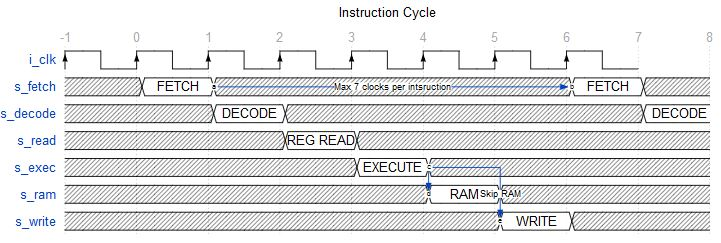
\includegraphics[scale=0.8]{td_instr}
\end{center}
\caption{The Discrete Fourier Transform definition \citep{wikipedia:dft}.}
\label{fig:dft_algorithm}
\end{figure}

\subsection{General Instructions} \label{sect:isa_general}
The term, general instruction, is given to instructions that are common to primitive operations such as arithmetic and comparison instructions.


\subsubsection{NOP}
\begin{description}[align=right,labelwidth=4cm]
\item [Description] The NOP instruction performs no action for 1 instruction cycle (see section  \ref{sect:isa_timings}).
\item [Assembly] NOP
\item [Pseudocode]
\item [Registers altered]
\item [Clock cycles] 2 (FETCH, DECODE)
\end{description}

\begin{table}[h]
\def\arraystretch{1.5}%  1 is the default, change whatever you need
    \begin{tabularx}{\textwidth}{|p{4cm}|X|}
    \hline
    15:11 & 10:0 \\
	\specialrule{2pt}{-2pt}{0pt}
	00000 & X
	\\ \hline
    \end{tabularx}
\end{table}


\subsubsection{LW - Load Word}
\begin{description}[align=right,labelwidth=4cm]
\item [Description] Copies a 16-bit word from RAM to a register.
\item [Assembly] LW
\item [Pseudocode] Rd $<=$ RAM[Ra + Simm5]
\item [Registers altered] Rd
\item [Clock cycles] 6 (FETCH, DECODE, READ, EXECUTE, RAM, WRITE)
\end{description}

\begin{table}[H]
\def\arraystretch{1.5}%  1 is the default, change whatever you need
    \begin{tabularx}{\textwidth}{|p{4cm}|p{2cm}|p{2cm}|X|}
    \hline
    15:11 & 10:8 & 7:5 & 4:0 \\
	\specialrule{2pt}{-2pt}{0pt}
	00001 & Rd & Ra & Simm5
	\\ \hline
    \end{tabularx}
\end{table}

\subsubsection{MOVR}
\begin{description}[align=right,labelwidth=4cm]
\item [Description] The MOVR instruction copies a 16-bit register value to another register.
\item [Assembly] MOVR \%Ra, \%Rd 
\item [Pseudocode] Rd $<=$ Ra
\item [Registers altered] Rd
\item [Clock cycles] 5 (FETCH, DECODE, READ, EXECUTE, WRITE)
\end{description}

\begin{table}[H]
\def\arraystretch{1.5}%  1 is the default, change whatever you need
    \begin{tabularx}{\textwidth}{|p{4cm}|p{2cm}|p{2cm}|X|}
    \hline
    15:11 & 10:8 & 7:5 & 4:0 \\
	\specialrule{2pt}{-2pt}{0pt}
	00011 & Rd & Ra & X
	\\ \hline
    \end{tabularx}
\end{table}

\subsubsection{MOVI}
\begin{description}[align=right,labelwidth=4cm]
\item [Description] The MOVR instruction copies a 16-bit register value to another register.
\item [Assembly] MOVR \%Ra, \%Rd 
\item [Pseudocode] Rd $<=$ Ra
\item [Registers altered] Rd
\item [Clock cycles] 5 (FETCH, DECODE, READ, EXECUTE, WRITE)
\end{description}

\begin{table}[H]
\def\arraystretch{1.5}%  1 is the default, change whatever you need
    \begin{tabularx}{\textwidth}{|p{4cm}|p{3cm}|X|}
    \hline
    15:11 & 10:8 & 7:0 \\
	\specialrule{2pt}{-2pt}{0pt}
	00100 & Rd & Imm8
	\\ \hline
    \end{tabularx}
\end{table}


\subsubsection{ADD}
\begin{description}[align=right,labelwidth=4cm]
\item [Description] The ADD instruction adds an immediate value to a destination register, Rd.
\item [Assembly] ADDI \$255, \%Rd
\item [Pseudocode]Rd $<=$ Rd + Imm8
\item [Registers altered] Rd
\item [Clock cycles] 5 (FETCH, DECODE, READ, EXEC, WRITE)
\end{description}

\begin{table}[H]
\def\arraystretch{1.5}%  1 is the default, change whatever you need
    \begin{tabularx}{\textwidth}{|p{4cm}|p{2cm}|p{2cm}|X|}
    \hline
    15:11 & 10:8 & 7:5 & 4:0 \\
	\specialrule{2pt}{-2pt}{0pt}
	01000 & Rd & Ra & X
	\\ \hline
    \end{tabularx}
\end{table}

\subsubsection{ADDI}
\begin{description}[align=right,labelwidth=4cm]
\item [Description] The ADD instruction adds an immediate value to a destination register, Rd.
\item [Assembly] ADDI \$255, \%Rd
\item [Pseudocode]Rd $<=$ Rd + Imm8
\item [Registers altered] Rd
\item [Clock cycles] 5 (FETCH, DECODE, READ, EXEC, WRITE)
\end{description}

\begin{table}[H]
\def\arraystretch{1.5}%  1 is the default, change whatever you need
    \begin{tabularx}{\textwidth}{|p{4cm}|p{3cm}|X|}
    \hline
    15:11 & 10:8 & 7:0 \\
	\specialrule{2pt}{-2pt}{0pt}
	01001 & Rd & Imm8
	\\ \hline
    \end{tabularx}
\end{table}


\subsubsection{SUBI}
\begin{description}[align=right,labelwidth=4cm]
\item [Description] The SUB instruction subtracts an immediate value from a destination register, Rd.
\item [Assembly] SUBI \$255, \%Rd
\item [Pseudocode]Rd $<=$ Rd - Imm8
\item [Registers altered] Rd
\item [Clock cycles] 5 (FETCH, DECODE, READ, EXEC, WRITE)
\end{description}

\begin{table}[H]
\def\arraystretch{1.5}%  1 is the default, change whatever you need
    \begin{tabularx}{\textwidth}{|p{4cm}|p{3cm}|X|}
    \hline
    15:11 & 10:8 & 7:0 \\
	\specialrule{2pt}{-2pt}{0pt}
	01001 & Rd & Imm8
	\\ \hline
    \end{tabularx}
\end{table}


\subsubsection{CMP}
\begin{description}[align=right,labelwidth=4cm]
\item [Description] Sets register, Rd, to the value of Ra - Rb.
\item [Assembly] CMP \%Ra, %Rd
\item [Pseudocode]Rd $<=$ CMP(Ra, Rd)
\item [Registers altered] Rd
\item [Clock cycles] 5 (FETCH, DECODE, READ, EXEC, WRITE)
\end{description}

\begin{table}[H]
\def\arraystretch{1.5}%  1 is the default, change whatever you need
    \begin{tabularx}{\textwidth}{|p{4cm}|p{2cm}|p{2cm}|p{2cm}|X|}
    \hline
    15:12 & 11:9 & 8:6 & 5:3 & 2:0 \\
	\specialrule{2pt}{-2pt}{0pt}
	0003 & Rd & Ra & Rb & X
	\\ \hline
    \end{tabularx}
\end{table}

\subsection{Special Instructions}

\newpage
\section{Compiler}
\subsection{}


\newpage
\bibliography{prco304} 
\end{document}
